\documentclass[../analysisII_notes.tex]{subfiles}
\begin{document}
\section{Aula 15 - 05 de Maio, 2025}
\subsection{Motivações}
\begin{itemize}
	\item Integração por Partes;
	\item Série de Taylor com Resto Integral;
	\item Sequências e Séries de Funções: a introdução.
\end{itemize}
\subsection{Teoremas Clássicos do Cálculo - Parte II.}
\begin{exr}
	Use o Teorema Fundamental do Cálculo para provar que a primeira Lei de Newton é consequência da Segunda Lei de Newton!
\end{exr}
\begin{tcolorbox}[
		skin=enhanced,
		title=Lembrete!,
		after title={\hfill Classes de Funções Diferenciáveis},
		fonttitle=\bfseries,
		sharp corners=downhill,
		colframe=black,
		colbacktitle=yellow!75!white,
		colback=yellow!30,
		colbacklower=black,
		coltitle=black,
		%drop fuzzy shadow,
		drop large lifted shadow
	]
	Dado intervalos I e J da reta, dizemos que uma função \(f:I\rightarrow J\) é de classe \(\mathcal{C}^{n}(I;J)\) se ela possui todas as suas n derivadas e elas são contínuas. Quando ela é infinitamente derivável, denotamos por \(\mathcal{C}^{\infty}(I;J)\) e, se for apenas contínua, pode ser escrita como \(\mathcal{C}^{0}(I;J).\)
\end{tcolorbox}

\hypertarget{integration_by_parts}{\begin{theorem*}[Integração por Partes.]
		Sejam \(f,\;g:[a, b]\rightarrow \mathbb{R}\) duas funções definidas no intervalo \([a, b]\) e de classe \(\mathcal{C}^{1}\). Vale que
		\[
			\int_{a}^{b}f'g \mathrm{dx} = fg \biggl|_{a}^{b}\biggr. - \int_{a}^{b}fg' \mathrm{dx}
		\]
	\end{theorem*}}
\begin{proof*}
	Com efeito, note que o produto \(f \cdot g\) é primitiva, pela Regra de Leibniz, de
	\[
		\frac{\mathrm{d}(fg)}{\mathrm{d}x} = fg' + f'g.
	\]
	Consequentemente, pelo \hyperlink{ftc}{\textit{Teorema Fundamental do Cálculo}}, temos
	\[
		fg \biggl|_{a}^{b}\biggr. = (fg)(b)-(fg)(a) = \int_{a}^{b}(f'g+fg') \mathrm{dx} = \int_{a}^{b}f'g \mathrm{dx} + \int_{a}^{b}fg' \mathrm{dx}.
	\]
	Portanto,
	\[
		\int_{a}^{b}f'g \mathrm{dx}fg \biggl|_{a}^{b}\biggr. - \int_{a}^{b}fg' \mathrm{dx}. \quad \text{\qedsymbol}
	\]
\end{proof*}
\begin{figure}[H]
	\begin{center}
		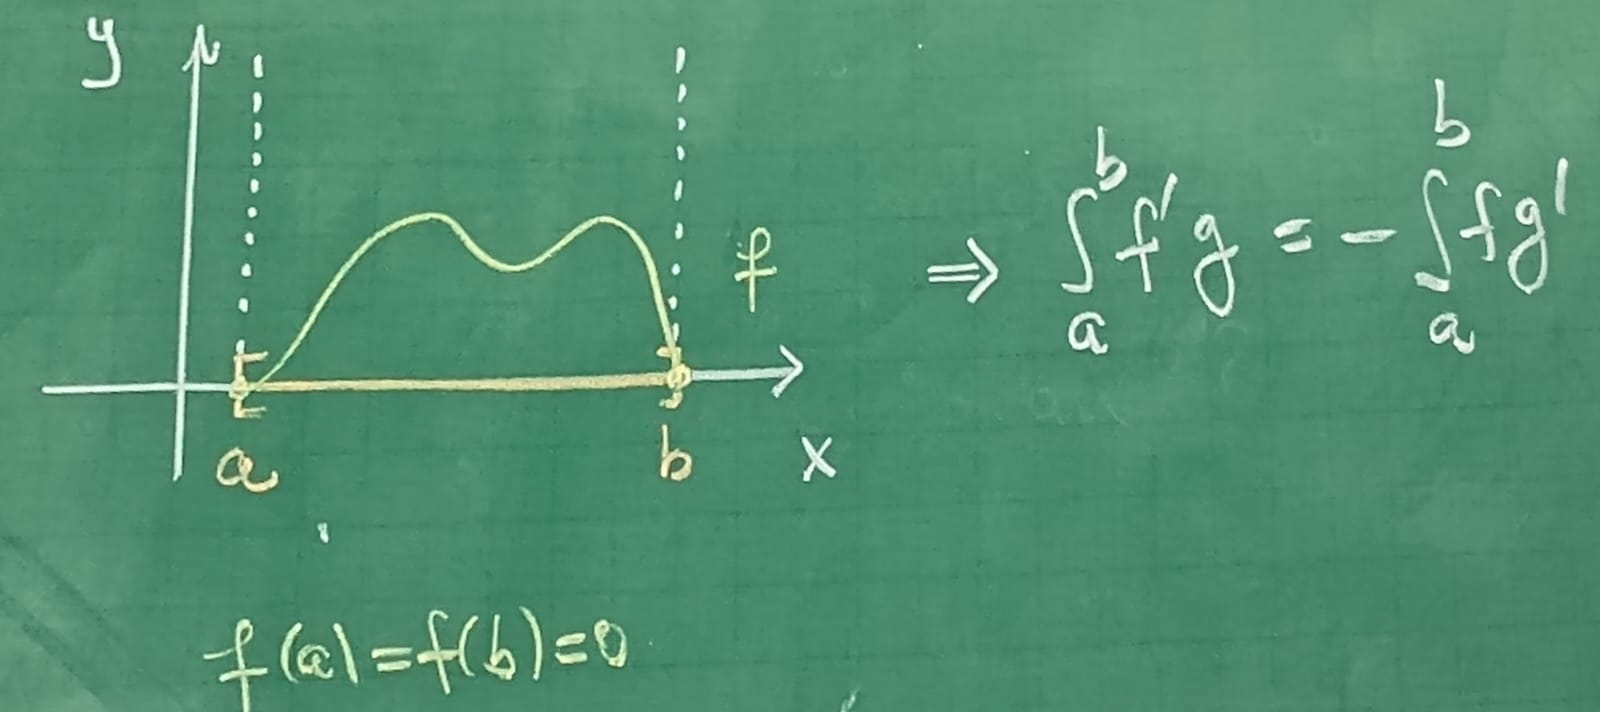
\includegraphics[height=0.4\textheight, width=0.4\textwidth, keepaspectratio]{./Images/integral_by_parts_15.png}
	\end{center}
	\caption{quando os pontos finais e iniciais da função no intervalo coincidem, a fórmula da integral por partes passa a ser simétrica!}
	\label{ibp15}
\end{figure}

\hypertarget{lemma_taylor}{
	\begin{lemma*}
		Seja \(\varphi \) uma função de classe \(\mathcal{C}^{n}([0, 1])\) para n natural. Então:
		\begin{align*}
			\varphi (1) & = \varphi (0) +\varphi '(0) + \frac{\varphi ''(0)}{2} + \dotsc + \frac{\varphi^{(n-1)}(0)}{(n-1)!} + \int_{0}^{1}\frac{(1-t)^{n-1}}{(n-1)!}\varphi^{(n)}(t) \mathrm{dt} \\
			            & = \sum\limits_{i=1}^{n-1}\frac{\varphi^{(i)}(0)}{i!} + \int_{0}^{1}\frac{(1-t)^{n-1}}{(n-1)!}\varphi^{(n)}(t) \mathrm{dt}.
		\end{align*}
	\end{lemma*}
}
\begin{proof*}
	A prova segue por indução no número de derivadas. O caso base de n = 1 nada mais é do que o Teorema Fundamental do Cálculo, pois
	\[
		\varphi (1) = \varphi (0) + \int_{0}^{1}\varphi '(t) \mathrm{dt} \Rightarrow \varphi (1)-\varphi (0) = \int_{0}^{1}\varphi '(t) \mathrm{dt},
	\]
	e a integral podemos reescrever como
	\[
		\int_{0}^{1}\varphi '(t) \mathrm{dt} = \int_{0}^{1}\frac{(1-t)^{1-1}}{(1-1)!}\varphi (1)(t) \mathrm{dt}.
	\]
	Logo, o caso base está provado.

	Supondo, agora, que a fórmula é válida para o n-ésimo caso, vamos mostrar para o (n+1)-ésimo. Com efeito, escreva:
	\[
		\varphi (1) = \sum\limits_{i=0}^{n-1}\frac{\varphi^{(i)(0)}}{i} + \int_{0}^{1}\frac{(1-t)^{n-1}}{(n-1)!}\varphi^{(n)}(t) \mathrm{dt}.
	\]
	Note que o termo multiplicando a n-ésima derivada de \(\varphi \) pode ser escrito como uma derivada:
	\[
		\frac{(1-t)^{n-1}}{(n-1)!} = \frac{\mathrm{d}}{\mathrm{d}t}\biggl[-\frac{(1-t)^{n}}{n!}\biggr],
	\]
	tal que, usando a integração por partes,
	\begin{align*}
		\varphi (1) & = \sum\limits_{i=0}^{n-1}\frac{\varphi^{(i)}(0)}{i!} - \biggl[\frac{(1-t)^{n}}{n!}\varphi^{(n)}\biggl|_{0}^{1}\biggr. - \int_{0}^{1}\frac{(1-t)^{n}}{n!}\varphi^{(n+1)}(t) \mathrm{dt}\biggr] \\
		            & = \sum\limits_{i=0}^{n-1}\frac{\varphi^{(i)}(0)}{i!} + \frac{\varphi^{(n)}(0)}{n!}+\int_{0}^{1}\frac{(1-t)^{n}}{n!}\varphi^{(n+1)}(t) \mathrm{dt}                                             \\
		            & = \sum\limits_{i=0}^{n}\frac{\varphi^{(i)}(0)}{i!} +\int_{0}^{1}\frac{(1-t)^{n}}{n!}\varphi^{(n+1)}(t) \mathrm{dt},
	\end{align*}
	como queríamos. \qedsymbol
\end{proof*}

\hypertarget{taylor_formula}{
	\begin{theorem*}[Fórmula de Taylor com Resto Integral]
		Se \(f:[a-\delta , a+\delta ]\rightarrow \mathbb{R}\) é de classe \(\mathcal{C}^{n}([a-\delta , a+\delta ])\) para algum \(\delta \) positivo (a f está definida ao redor do ponto a, onde faremos a expansão), então para todo x nesta vizinhança-\(\delta \) de a, tem-se
		\[
			f(x) =\sum\limits_{i=0}^{n-1}\frac{f^{(i)}(a)}{i!}(x-a)^{i} + (x-a)^{n}\int_{0}^{1}\frac{(1-t)^{n-1}}{(n-1)!}f^{(n)}(a+t(x-a)) \mathrm{dt}.
		\]
		Aqui, x é a \textbf{variável}, o termo integral é o chamado \textbf{resto integral} e a série é o chamado \textbf{polinômio de Taylor da função f de ordem (n-1) em a}.
	\end{theorem*}
}
\begin{proof*}
	Basta definir \(\varphi :[0, 1]\rightarrow \mathbb{R}\) pondo, para cada x no intervalo \([a-\delta , a+\delta ]\),
	\[
		\varphi (t)\coloneqq f(a+t(x-a)),\quad t\in[0, 1].
	\]
	Como a f é de classe \(\mathcal{C}^{n}\) e a equação da reta à qual ela está sendo aplicada também é\footnote{Na verdade, é suave!}, a própria \(\varphi \) também é, e podemos aplicar a regra da cadeia
	\begin{align*}
		 & \varphi '(t) = f'(a+t(x-a))(x-a)               \\
		 & \varphi''(t) = f''(a+t(x-a))(x-a)^{2}          \\
		 & \vdots                                         \\
		 & \varphi^{(n)}(t) = f^{(n)}(a+t(x-a))(x-a)^{n}.
	\end{align*}
	Calculando isso no zero, segue que
	\begin{align*}
		 & \varphi '(0) = f'(a)(x-a)               \\
		 & \varphi''(0) = f''(a)(x-a)^{2}          \\
		 & \vdots                                  \\
		 & \varphi^{(n)}(0) = f^{(n)}(a)(x-a)^{n},
	\end{align*}
	donde, substituindo a \(\varphi\) na fórmula do \hyperlink{lemma_taylor}{\textit{Lema}}, chegamos em
	\[
		\varphi^{(i)}(0) = \frac{\varphi^{(i)}(a)}{i!}(x-a)^{i}.
	\]
	Sabendo que \(\varphi (1) = f(x)\), basta substituir de novo na fórmula do \hyperlink{lemma_taylor}{\textit{Lema}}, provando o teorema. \qedsymbol
\end{proof*}
Aqui, demarcamos o fim do tópico de integração!

\subsection{Sequências e Séries de Funções}
Existem várias formas para começar esta parte do curso: pela física, olhando para o problema da mecânica clássica (Newton + Hamilton), observa-se que suas leis costumam ser formuladas por EDO's, principalmente devido à segunda lei de Newton
\[
	F(x) = m \ddot{x}(t).
\]
Nela, temos as ``leis verdadeiras''\footnote{Dizia Newton que eram criadas por Deus.}, como
\[
	f(x) = \dot{x},
\]
e as ``leis aproximadas'', que são as que conseguimos detectar dadas as limitações humanas, com erros e aproximações:
\[
	\dot{x}_{n} = f_{n}(x_{n}).
\]
Fica a pergunta: como podemos dizer que a lei aproximada é de fato uma aproximação da Lei Verdadeira? E é possível resolver a lei aproximada tal que ela aproxime o melhor possível as Leis Verdadeiras?

A segunda, (adicionada em breve)

Com isto, vamos pôr a mão na massa e definir nossa primeira coisa
\begin{def*}
	Dado um subconjunto X da reta real, uma sequência de funções em X é uma correspondência que associa a cada natural n uma função \(f_{n}:X\rightarrow \mathbb{R}\) definida em X. Nestas condições, escreveremos ``\(f_{n}:X\rightarrow \mathbb{R},\; n\in \mathbb{N}\)'' ou, se o domínio for fixo, ``\(\{f_{n}\}_{n\in \mathbb{N}}\)'', ou até mesmo
	\[
		X\ni x \mapsto f_{n}(x),\quad n\in \mathbb{N}.\quad \square
	\]
\end{def*}
\begin{figure}[H]
	\begin{center}
		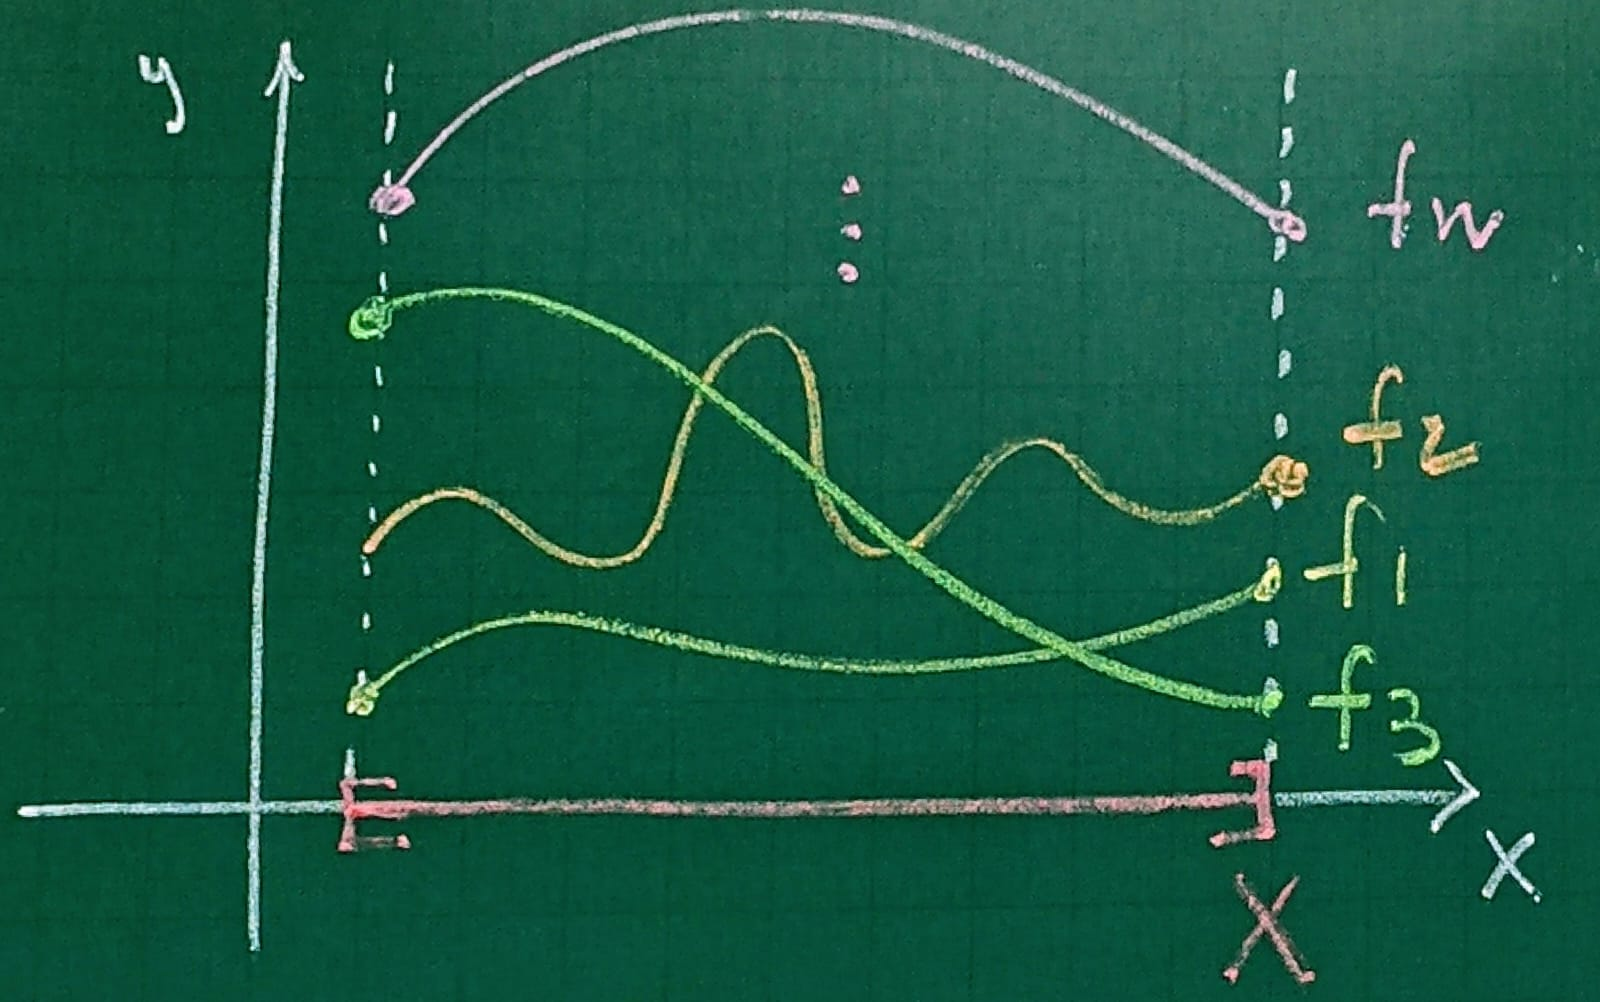
\includegraphics[height=0.5\textheight, width=0.5\textwidth, keepaspectratio]{./Images/sequence_functions_15.png}
	\end{center}
	\caption{cada função na sequência não precisam estar relacionadas entre si!}
	\label{seq15}
\end{figure}
\begin{tcolorbox}[
		skin=enhanced,
		title=Observação,
		fonttitle=\bfseries,
		colframe=black,
		colbacktitle=cyan!75!white,
		colback=cyan!15,
		colbacklower=black,
		coltitle=black,
		drop fuzzy shadow,
		%drop large lifted shadow
	]
	Dada uma ``sequência de funções'' \(f_{n}:X\rightarrow \mathbb{R}\), com n natural, vale que para cada ponto \(x_{0}\) em X, ela associa uma sequência de números reais
	\[
		f_1(x_{0}), f_2(x_{0}), \dotsc , f_{n}(x_{0}), \dotsc,
	\]
	para a qual existe a noção de limite. Portanto, podemos indagar sobre a existência do limite
	\[
		\lim_{n\to \infty}\overbrace{f_{n}(x_{0})}^{\mathclap{a_{n}\in \mathbb{R}}}.
	\]
	Com isso, o conjunto dos pontos para os quais a sequência converge torna-se um objeto de estudo interessante, criando o primeiro conceito de convergência - a pontual - que iremos estudar.
\end{tcolorbox}
\begin{def*}
	Dada uma sequência de funções \(f_{n}:X\rightarrow \mathbb{R}\), dizemos que \textbf{a sequência converge pontualmente em x de X para uma função f com domínio X} (ponto-a-ponto/simplesmente), \(f:X\rightarrow \mathbb{R}\), se para cada ponto x de X, a sequência de números
	\[
		(f_{n}(x))_{n\in \mathbb{N}}
	\]
	converge em \(\mathbb{R}\) para o valor f(x). Escreveremos
	\[
		f_{n}\overbracket[0pt]{\longrightarrow}_{n\to \infty}^{p}f. \square
	\]
\end{def*}
\begin{example}
	\begin{itemize}
		\item[1)] Considere \(X = \mathbb{R}\) e a sequência com membros dados por
		      \[
			      f_{n}(x) = \frac{x}{n},\quad n\in \mathbb{N}.
		      \]
		      Temos uma sequência de retas passando pela origem e com inclinação \(\dfrac{1}{n}\).
		      \begin{figure}[H]
			      \begin{center}
				      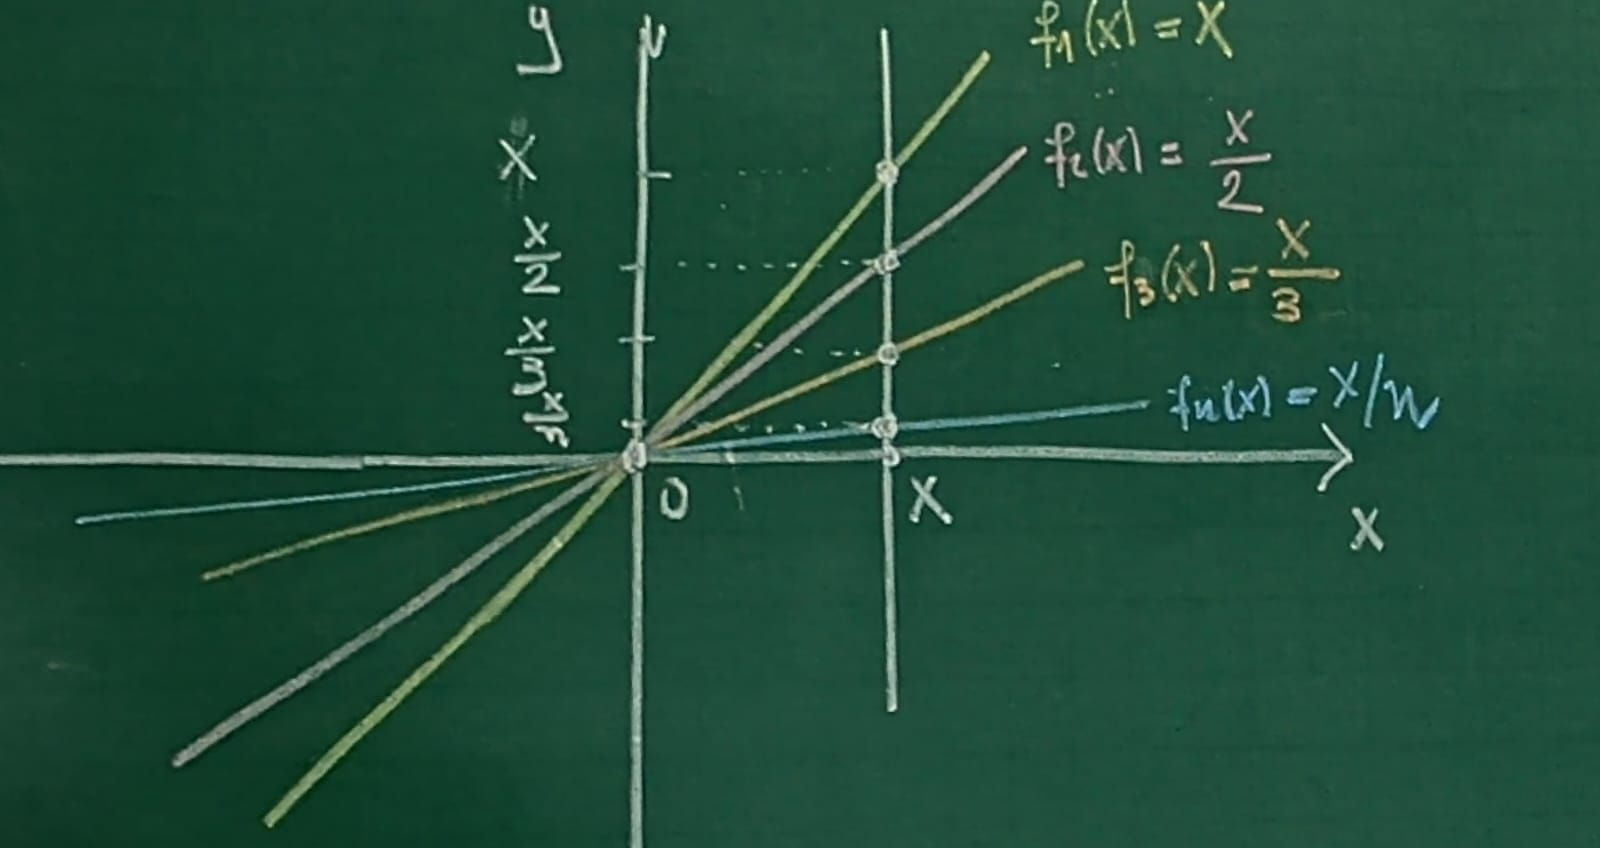
\includegraphics[height=0.5\textheight, width=0.5\textwidth, keepaspectratio]{./Images/inclined_sequence_15.png}
			      \end{center}
			      \caption{cada n ``aumenta a inclinação'' das funções, até que o limite fica uma reta no eixo x - uma reta constantemente nula!}
			      \label{inc15}
		      \end{figure}
	\end{itemize}
\end{example}
\end{document}
